\documentclass[a4paper,DIV=12,english]{scrartcl}
\usepackage[utf8]{inputenc}
\usepackage{fancyhdr}
\usepackage{bookmark}
\usepackage{graphicx}
\usepackage{hyperref}
\usepackage{xurl}
\usepackage[sorting=none, style=numeric-comp]{biblatex}
\addbibresource{ref.bib}
\usepackage{csquotes}
\usepackage[dvipsnames]{xcolor}
\usepackage[num]{isodate}
\usepackage{amsthm}
\usepackage{amssymb}
\usepackage{bbm}
\usepackage{amsmath}
\usepackage{tikz}
%\usepackage{pgfplots}
    %\usepgfplotslibrary{fillbetween}
\usepackage{svg}
\usepackage{braket}
\usepackage{caption}
\usepackage{subcaption}
\usepackage{placeins}
%\setlength\parindent{0pt}
\usepackage{wrapfig}
\usepackage{float}


% Fakesection
\newcommand{\fakesection}[1]{%
    \par\refstepcounter{section}                                        % Increase section counter
    \sectionmark{#1}                                                    % Add section mark (header)
    \addcontentsline{toc}{section}{\protect\numberline{\thesection}#1}  % Add section to ToC
    % Add more content here, if needed.
} 

\renewcommand{\footrulewidth}{0.5pt}
\pagestyle{fancy}
\fancyhf{}
\fancyhead[L]{\leftmark}
\fancyhead[R]{}

\fancyfoot[C]{Computational Physics: Alpha Decay}
\fancyfoot[R]{\thepage}

\title{Computational Physics: Alpha Decay Project Report}
\author{Stockholm University, Spring Term 2024 \\Max Maschke}
\date{Mar 26 2024}


\begin{document}
\maketitle


\tableofcontents
\newpage


\newpage
\section{Introduction}

\section{Alpha Decay}
Alpha decay is the process in which a nucleus $^A_Z \text{X}$ emits an alpha particle $^4\text{He}^{2+}$, leaving behind a $^{A-4}_{Z-2}\text{Y}$ nucleus. This mode of decay occurs mostly in heavy nuclei such as $^{238} \text{U}$, which decays into $^{234}\text{Th}$. Generally, alpha decay can only occur if the combined energy of the alpha particle and the daughter nucleus is less than that of the original nucleus, i.e.
\begin{equation}
    M_\text{X} c^2 > (M_\text{Y} + M_\alpha)c^2
\end{equation}

Alpha decay can be understood as a quantum tunnelling effect in which the spontaneously created alpha particle has a non-zero probability to leave the nucleus, in which it is bound by the strong force, crossing the Coulomb wall and escaping. This naive view assumes that both the nucleus and the alpha particle have zero angular momentum. A further approximation used henceforth is to assume that all the energy released in the decay is converted to kinetical energy of the daughter particles, i.e.\ both particles are emitted in their respective ground states.

The task at hand is this to solve the Schrödinger equation for the wave function $\psi$,
\begin{equation}
    \left[-\frac{\hbar^2}{2M_\alpha} \partial_r^2 + V(r)\right] \psi(r) = E_\alpha \psi(r)\,,
\end{equation}
where $r$ is the radial coordinate taken from the centre of the nucleus and $V(r)$ is the spherically symmetrical potential that incorporates both the attracting close range nature of the strong force and the repelling Coulomb potential. The former is commonly taken to be constant up to the extension of the nucleus $R$, such that
\begin{equation}
    V(r) =  \begin{cases}
                - V_0 & r \leq R\\
                \alpha \hbar c\, \frac{Z_\text{Y}Z_\alpha}{r} & r > R
            \end{cases}\,,
\end{equation}
where $V_0$ is the depth of the strong force well, $\alpha$ is the fine structure constant, $Z_\alpha=2$ and $Z_\text{Y}$ is the proton number of the daughter nucleus. It must be stressed that the choice of $R$ is a key parameter of the model. Commonly, $R = \tilde R \cdot A^{1/3}$ is used where $\tilde R$ is a scaling factor in the vicinity of 1.3. This essentially assumes that the nucleus is spherical, however, this is not true especially for large nuclei which are actually deformed.

Note that since the goal is not to solve for bound states, $E_\alpha$ is a parameter of the equation that is obtained from the mass excess released in the decay. From the solution of the Schrödinger equation, one can obtain in principle the probability amplitude of the alpha particle outside the classically forbidden region, i.e.\ the region $r > R_\text{C}$ where $R_\text{C}$ is the radius given by solving
\begin{equation}
    E_\alpha = V(r)\,.
\end{equation}

Since an exact solution of the problem is not tractable, one must look for appropriate ways to find an approximate solution. One such way is to discretise the potential into evenly spaced regions in which the potential is taken to be constant. The solution of the 1D Schrödinger equation in regions of constant potential $V$ for a particle with energy $E$ is known and given by
\begin{equation}
    \psi(x) = A \text{e}^{kx} + B \text{e}^{-kx}
\end{equation}
where $A$ and $B$ are complex constants and $k=\sqrt{2M_\alpha(V-E)}/\hbar$. Note that if $E>V$, $k$ is complex and the solution is oscillating, while for $E<V$ the solution is exponentially decaying or growing depending on the relation of $A$ and $B$.

As the wave function must be continuously differentiable, the constants can be fixed by imposing appropriate analycity conditions at the boundaries between bins, that is for every connection point $x_i$, two conditions are obtained:
\begin{align}
    0 &= A_i \text{e}^{k_ix_i} + B_i \text{e}^{-k_ix_i} - A_{i+1} \text{e}^{k_{i+1}x_i} - B_{i+1} \text{e}^{-k_{i+1}x_i} \\
    0 &= k_iA_i \text{e}^{k_ix_i} - k_i B_i \text{e}^{-k_ix_i} - k_{i+1}A_{i+1} \text{e}^{k_{i+1}x_i} + k_{i+1} B_{i+1} \text{e}^{-k_{i+1}x_i} \\
\end{align}

For the case of alpha decay, $B=0$ can be chosen for the outgoing solution beyond $R_\text{C}$ as well as $A=1$ for the solution inside the nuclear well.

In principle, as the number of bins is taken to infinity, the solution should converge to the exact solution. 

While the quantity of chief interest is not the wave function but rather the half-life of different nuclei, this can be gained from the solution of the piecewise discretised potential by a semi-classical argument:

The alpha particle can be taken to be moving with velocity
\begin{equation}
    v_\alpha = \sqrt{2 \frac{E_\alpha}{M_\alpha} }\,,
\end{equation}
bouncing between the boundaries of the nucleus, which it hits with frequency $V_\alpha / 2R$. The decay constant $\tau$ is then 
\begin{equation}
    \tau = \frac{2R}{v T}
\end{equation}
where $T$ is the transmission coefficient obtained from the conservation of probability current:
\begin{equation}
    1 = |A_\text{well}|^2 = |B_\text{well}|^2 + \underbrace{|B_\text{out}|^2 \frac{k_\text{out}}{k_\text{in}}}_{=T}
\end{equation}
The half-life follows from the decay constant:
\begin{equation}
    t_{1/2} = \tau \ln 2
\end{equation}


\section{Numerical formulation}
\subsection{Linear system of equations}
Solving for the wave function constants reduces to solving a linear system (LSE) $Ax = b$:
\begin{equation}
    \begin{bmatrix}
        1 & & & & & & \dots \\
        \text{e}^{k_1 x_1} & \text{e}^{-k_1 x_1} & \text{e}^{k_2 x_1} & \text{e}^{-k_2 x_1} & & & \dots \\
        k_1\text{e}^{k_1 x_1} & -k_1\text{e}^{-k_1 x_1} & k_2\text{e}^{k_2 x_1} & -k_2\text{e}^{-k_2 x_1} & & & \dots \\
        & & \text{e}^{k_2 x_2} & \text{e}^{-k_2 x_2} & \text{e}^{k_3 x_2} & \text{e}^{-k_3 x_2} & \dots \\
        & & k_2\text{e}^{k_2 x_2} & -k_2\text{e}^{-k_2 x_2} & k_3\text{e}^{k_3 x_2} & -k_3\text{e}^{-k_3 x_2} & \dots \\
        & & & & {e}^{k_3 x_3} & \text{e}^{-k_3 x_3} & \dots \\
        \vdots & \vdots & \vdots & \vdots & \vdots & \vdots & \ddots 
    \end{bmatrix}
    \begin{bmatrix}
        A_1 \\
        B_1 \\
        A_2 \\
        B_2 \\
        A_3 \\
        B_3 \\
        \vdots
    \end{bmatrix}
    =
    \begin{bmatrix}
        1 \\
        0 \\
        0 \\
        0 \\
        0 \\
        0 \\
        \vdots
    \end{bmatrix}
\end{equation}
where the positions $x_i$ are given by 
\begin{equation}
    x_i = R + (i-1) dx,\quad i = 1, \dots, N
\end{equation}
with $dx = \frac{R_\text{C} - R}{N}$ and $N$ the number of bins. The $k_i$ are the $k$ from above evaluated at $V = V_i$, such that $V_0 = V_0$ and $V_{i\neq 0} = V(x_i)$.

This approach causes an issue: since $R_\text{C}$ was chosen such that $V(R_\text{C}) = E_\alpha$, $k_N = 0$ which implies $T = 0$. This is remedied by imposing a slight offset onto the last discretised position $x_N = R + (N-1) dx + \epsilon$ with $\epsilon = 10^{-14}\,\text{fm}$.

The solution to the LSE is obtained by numerically calculating the LU decomposition of $A$
\begin{equation}
    P A  = L U
\end{equation}
where $P$ is a permutation matrix, $L$ a lower triangular matrix with unit diagonal and $U$ an upper triangular matrix. If, for simplicity, $P = I$, substituting yields
\begin{equation}
    L (Ux) = b\,.
\end{equation}
This system is easy to solve for $y = Ux$ using forward substitution because of the structure of $L$. Similarly, it is easy to then solve $Ux = y$ using back substitution. Calculating the LU decomposition has complexity $O(n^3)$ where $n$ is the dimension of the matrix (obtaining the solution is then $O(n^2)$, which is why it is easy to get the solution for multiple right-hand sides once the LU decomposition has been obtained~\cite{numerik}).

\subsection{Units}
For the representation of the quantities position and energy, femtometres (fm) and MeV are used, respectively. It is convenient to then use mass-energy equivalents $Mc^2$ instead of the actual masses. For example, as noted in the lecture,
\begin{equation}
    k = \frac{1}{\hbar} \sqrt{2 M (V - E)} = \frac{1}{\hbar c} \sqrt{2 (Mc^2) (V - E)} 
\end{equation}
and, as noted above, $V = \alpha \hbar c / r$, so all unit conversions can be done using the two constants $\alpha$ and $\hbar c$.

\section{Implementation}
For this comparatively simple problem, Python is chosen for implementing the numerical scheme described above in. The bulk of the computational work that has to be done is the calculation of the LU decomposition, which is done using \texttt{Numpy}'s \texttt{linalg.solve} function~\cite{harris2020array}, which, in our case is a wrapper for \texttt{zgesv} from the \texttt{LAPACK} library~\cite{laug}. Since the LU decomposition is thus determined using compiled \texttt{FORTRAN} code, there is no major downside to using Python in terms of computational performance.

However, to optimize the performance beyond that of standard Python, we use the \texttt{Numba} package~\cite{numba} which allows for Python code to be just-in-time transpiled to C and then compiled, with some restrictions on the language features that can be used. The main expected benefit from this is when constructing the coefficient matrix, especially when many bins are used.

We implement a just-in-time compiled class \texttt{Alphadecay} that contains the functionality to build the coefficient matrix for a given element, solve the LSE and calculate the half-life. We also implement a number of functions to test the performance and numerics, as well as ones to visualise the results.

The code is enclosed with this report and also available at~\cite{github}.

\section{Results}
In the following section, the implemented solution of the alpha decay tunnelling problem is to be analysed as to its performance and numerical stability as well as the physical results.

\subsection{Performance}
First, the scaling of elapsed time to solve the LSE with the number of potential bins is to be looked at. The results of a simple empirical runtime analysis on an i7-1065G7 CPU are shown in \ref{fig:bench}. 

One can observe that for one added order of magnitude in the number of bins, the runtime rises by approximately three orders of magnitude, which is consistent with the $O(3)$ nature of the LU algorithm. 

Small deviations from the expected linear behaviour (on the logarithmic plot, that is) at small bin numbers can be attributed to lower order contributions to complexity and overhead, while for larger bin numbers, variations in system load may be the reason.
\begin{figure}
    \centering
    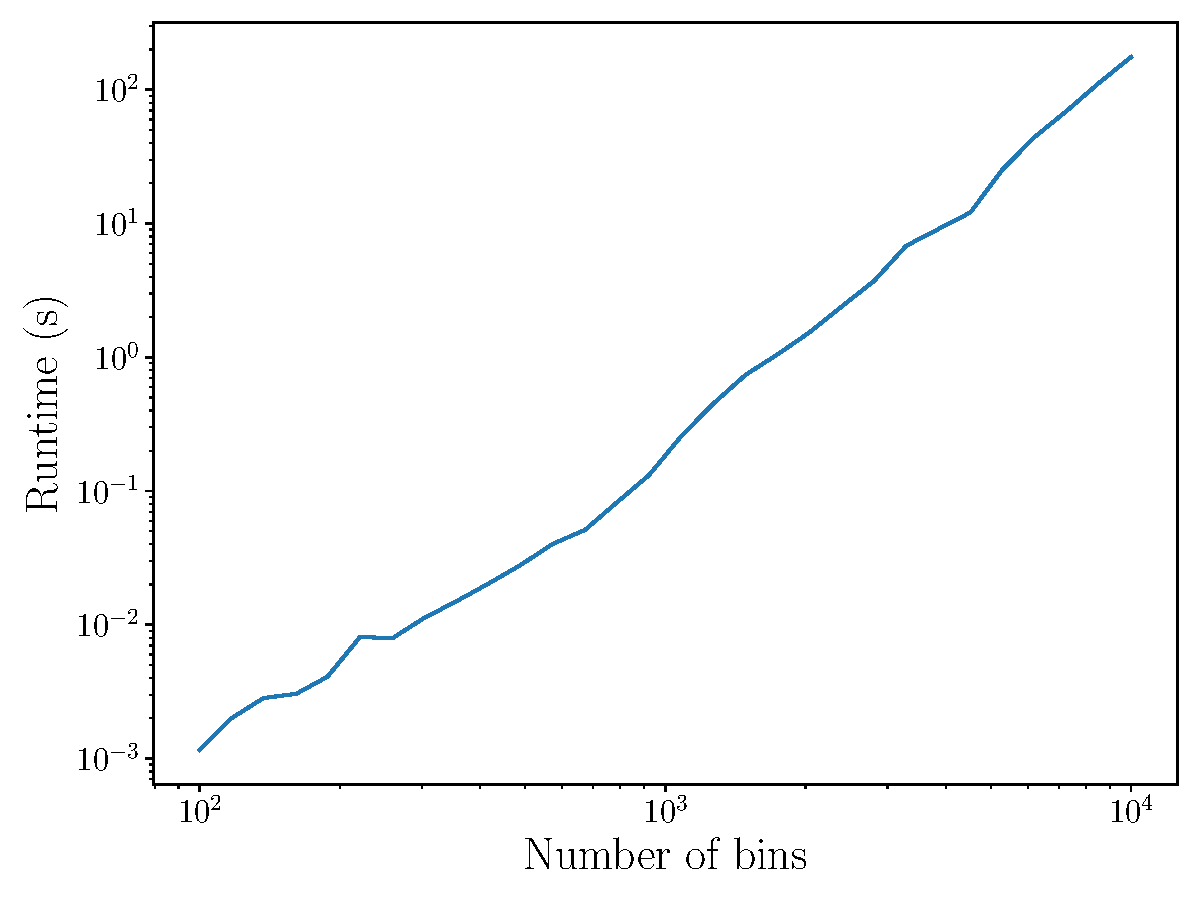
\includegraphics[width=0.5\textwidth]{../plots/runtime.pdf}
    \caption{Runtime scaling with the number of potential bins of the process of creating and solving the LSE for the coefficients. CPU: i7-1065G7. One can observe that for one added order of magnitude in the number of bins, the runtime rises by approximately three orders of magnitude, which is consistent with the $O(3)$ nature of the LU algorithm. Deviations in the graph can be attributed to lower order contributions and variations in system load.}
    \label{fig:bench}
\end{figure}

\subsection{Numerics}
To gain insight into the numeric performance of the implemented method, the dependence of the predicted half life on the number of potential bins used is shown for five isotopes in figure~\ref{fig:binsize}. 

It can be seen that the algorithm converges to a single value for all isotopes as $N$ is increased. This suggests that the algorithm is approaching the true solution of the problem, assuming that the implementation of the LSE is correct.

Comparing the plots for the different elements studied, a bin number of $N > 1000$ seems to be needed to reduce the approximation error to an acceptable amount. $N = 2000$ was chosen to obtain the final values presented later.
\begin{figure}
    \centering
    \begin{subfigure}{0.49\textwidth}
        \centering
        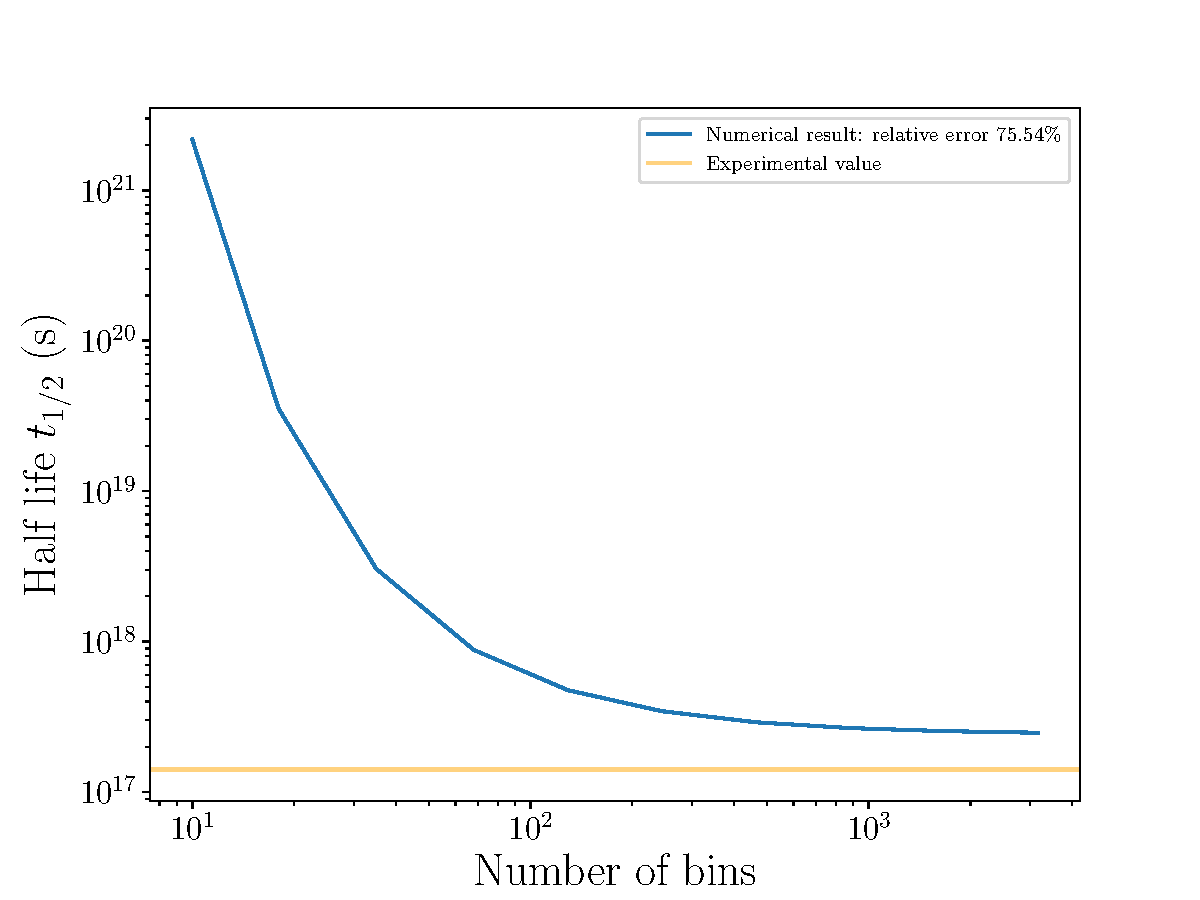
\includegraphics[width=0.9\textwidth]{../plots/bin_dependence/bins_u238.pdf}
        \caption{$^{238}\text{U}$}
        \label{subfig:bins_u238}
    \end{subfigure}
    \begin{subfigure}{0.49\textwidth}
        \centering
        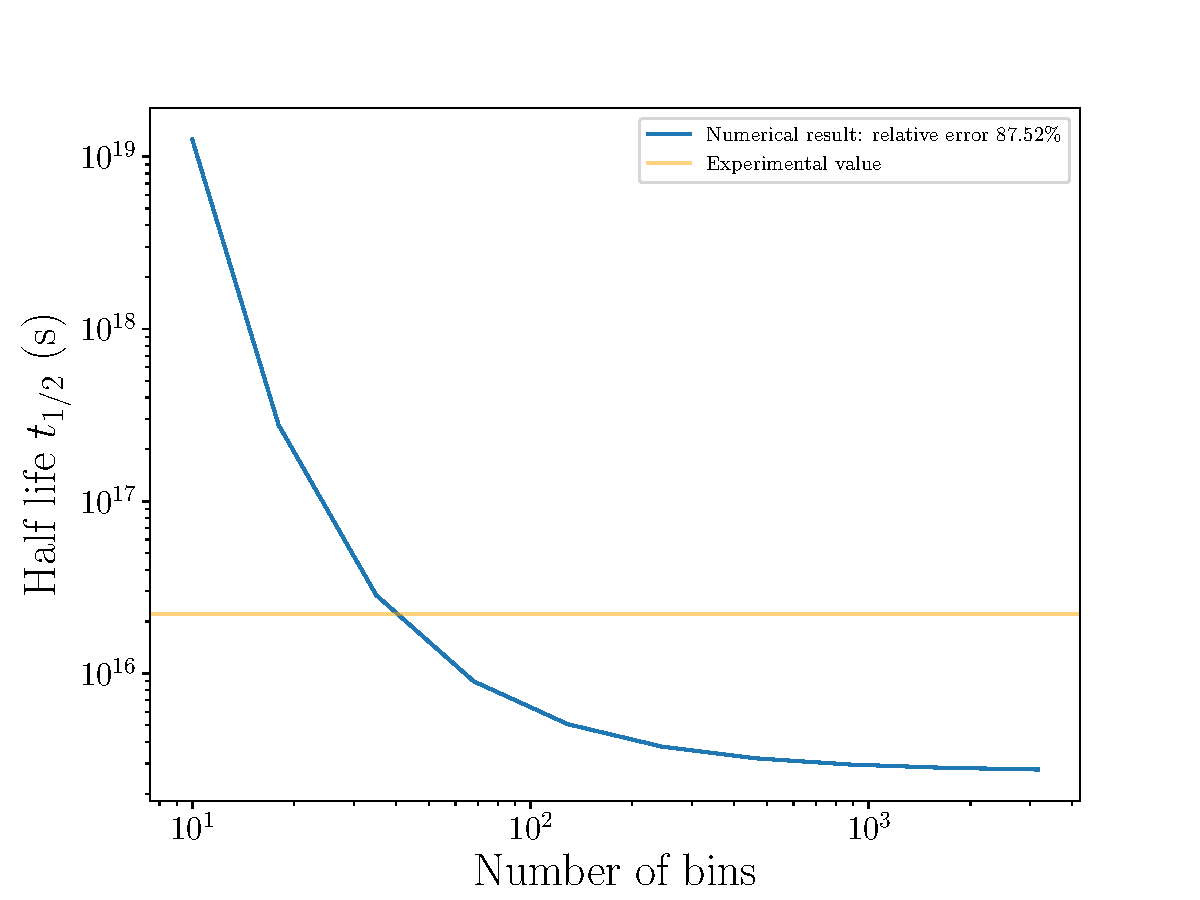
\includegraphics[width=0.9\textwidth]{../plots/bin_dependence/bins_u235.pdf}
        \caption{$^{235}\text{U}$}
        \label{subfig:bins_u235}
    \end{subfigure}\\
    \begin{subfigure}{0.49\textwidth}
        \centering
        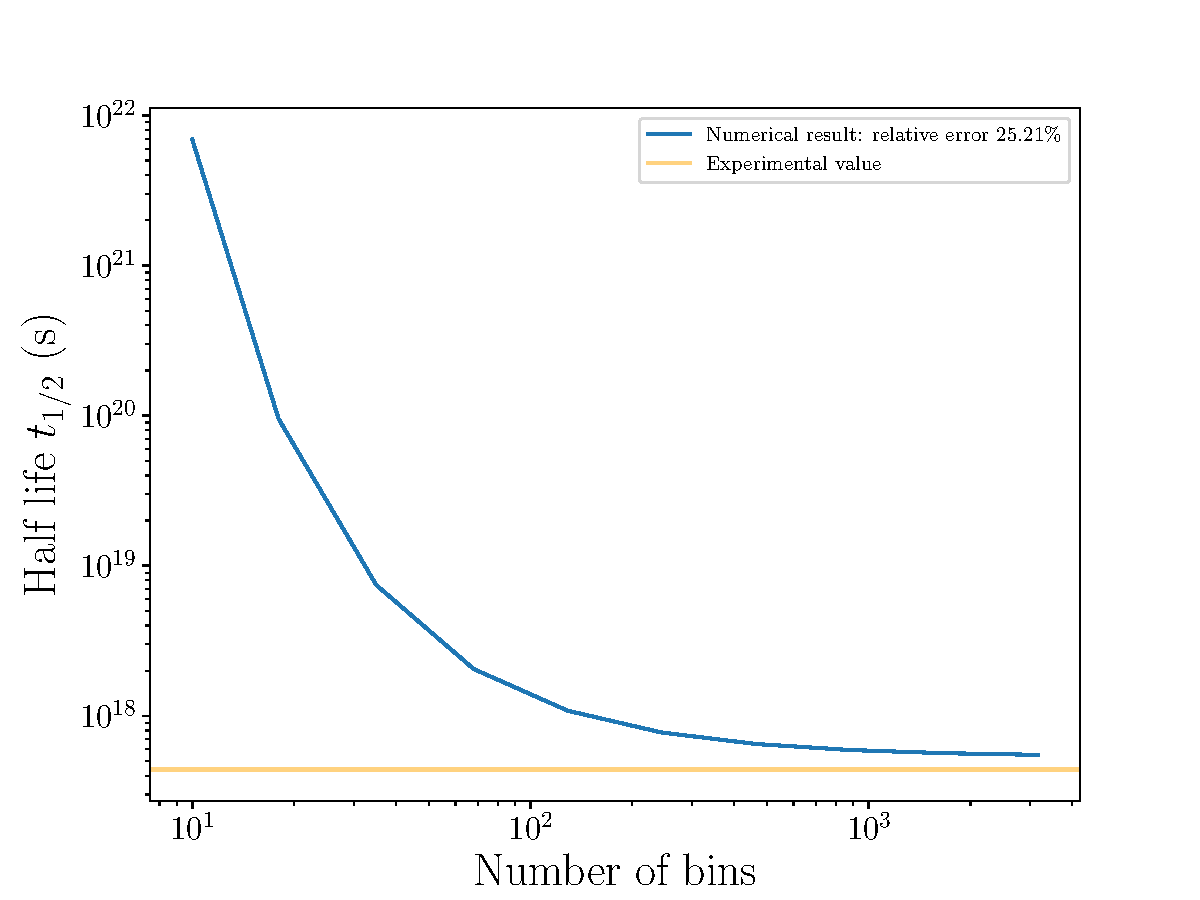
\includegraphics[width=0.9\textwidth]{../plots/bin_dependence/bins_th232.pdf}
        \caption{$^{232}\text{Th}$}
        \label{subfig:bins_th232}
    \end{subfigure}
    \begin{subfigure}{0.49\textwidth}
        \centering
        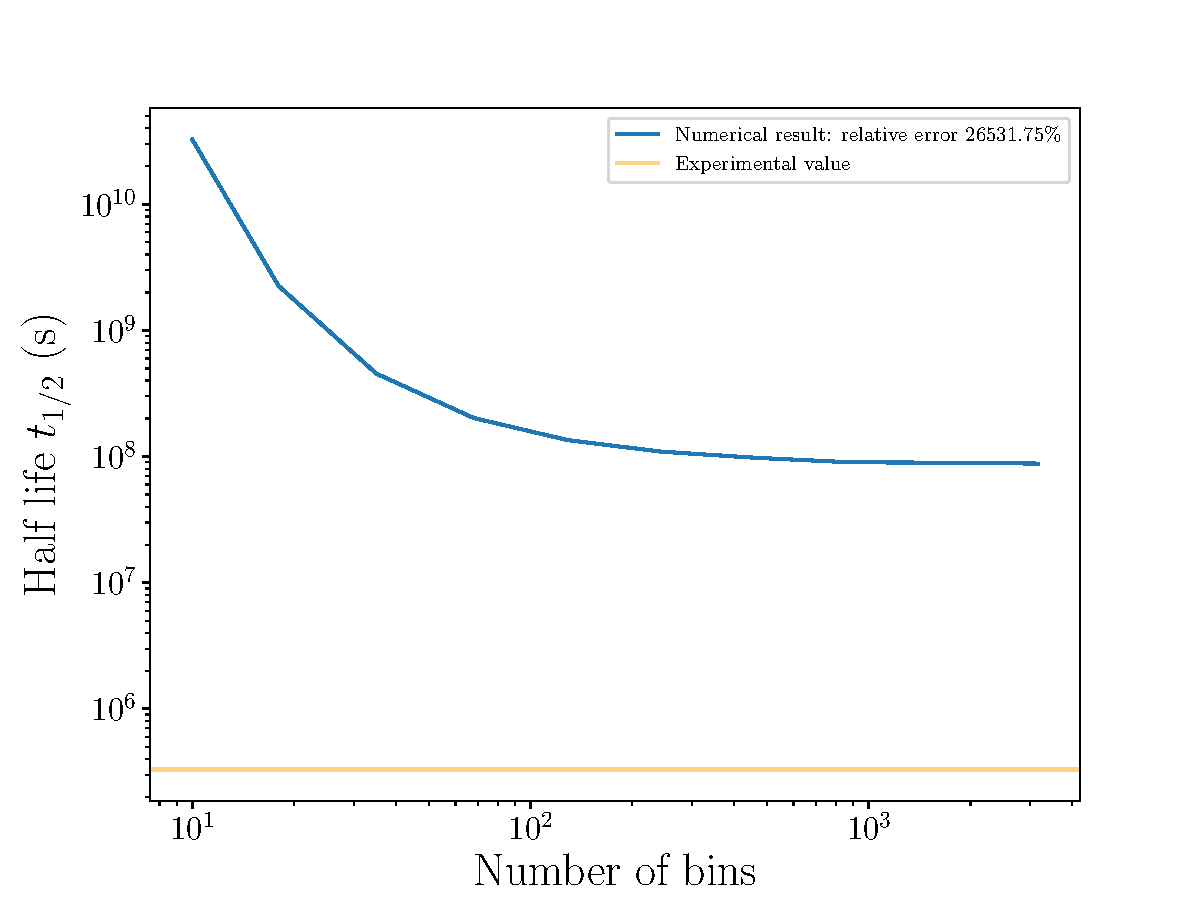
\includegraphics[width=0.9\textwidth]{../plots/bin_dependence/bins_rn222.pdf}
        \caption{$^{222}\text{Rn}$}
        \label{subfig:bins_rn222}
    \end{subfigure}\\
    \begin{subfigure}{0.49\textwidth}
        \centering
        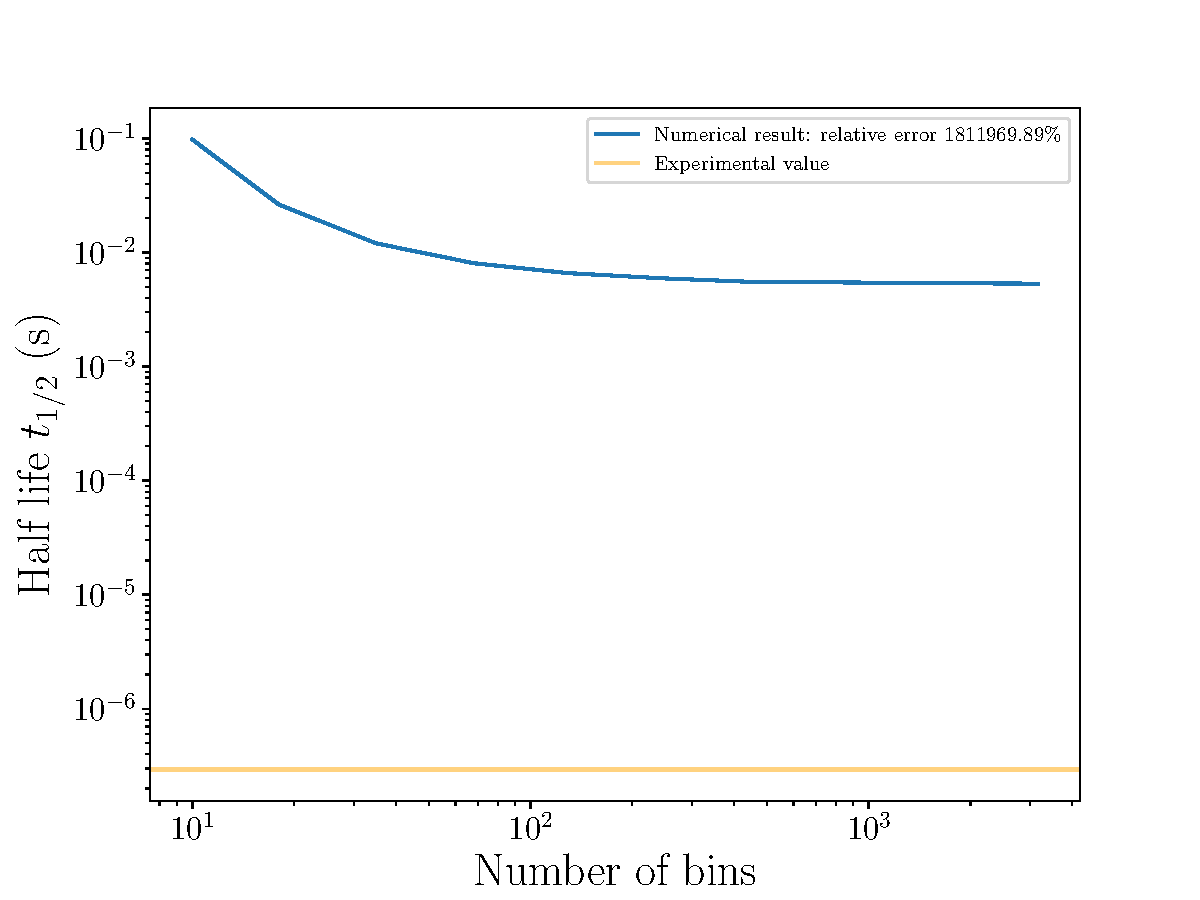
\includegraphics[width=0.9\textwidth]{../plots/bin_dependence/bins_po212.pdf}
        \caption{$^{212}\text{Po}$}
        \label{subfig:bins_po212}
    \end{subfigure}
    \caption{Convergence of the numerically estimated half life with increasing number of bins. Experimental values are shown for reference, for interpretation of the physics, refer to the next section. Convergence to a single value with increasing bin number is an encouraging sign that suggests that the algorithm approaches the true value of the posed problem. Comparing the plots for the different elements studied, a bin number of $N > 1000$ seems to be needed to reduce the approximation error to an acceptable amount.}
    \label{fig:binsize}
\end{figure}

The project description suggests investigating the numerical error of the solution obtained from the LU decomposition. Sadly, this has to be omitted here due to a lack of time ahead of the deadline. However, every obtained solution of the LSE was checked for validity using the criterion $||Ax - b|| < 10^{-5}$. $||Ax - b||$ was usually observed to be of order of $10^{-6}$ or less.

\subsection{Physics}
Five isotopes were decided on as test cases for the algorithm: $^{238}\text{U}$, $^{235}\text{U}$, $^{232}\text{Th}$, $^{222}\text{Rn}$ and $^{212}\text{Po}$. For these and their decay products, the atomic masses were obtained from \cite{Wolfram} which refers to \cite{Audi} as its source.

\begin{figure}
    \centering
    \begin{subfigure}{0.49\textwidth}
        \centering
        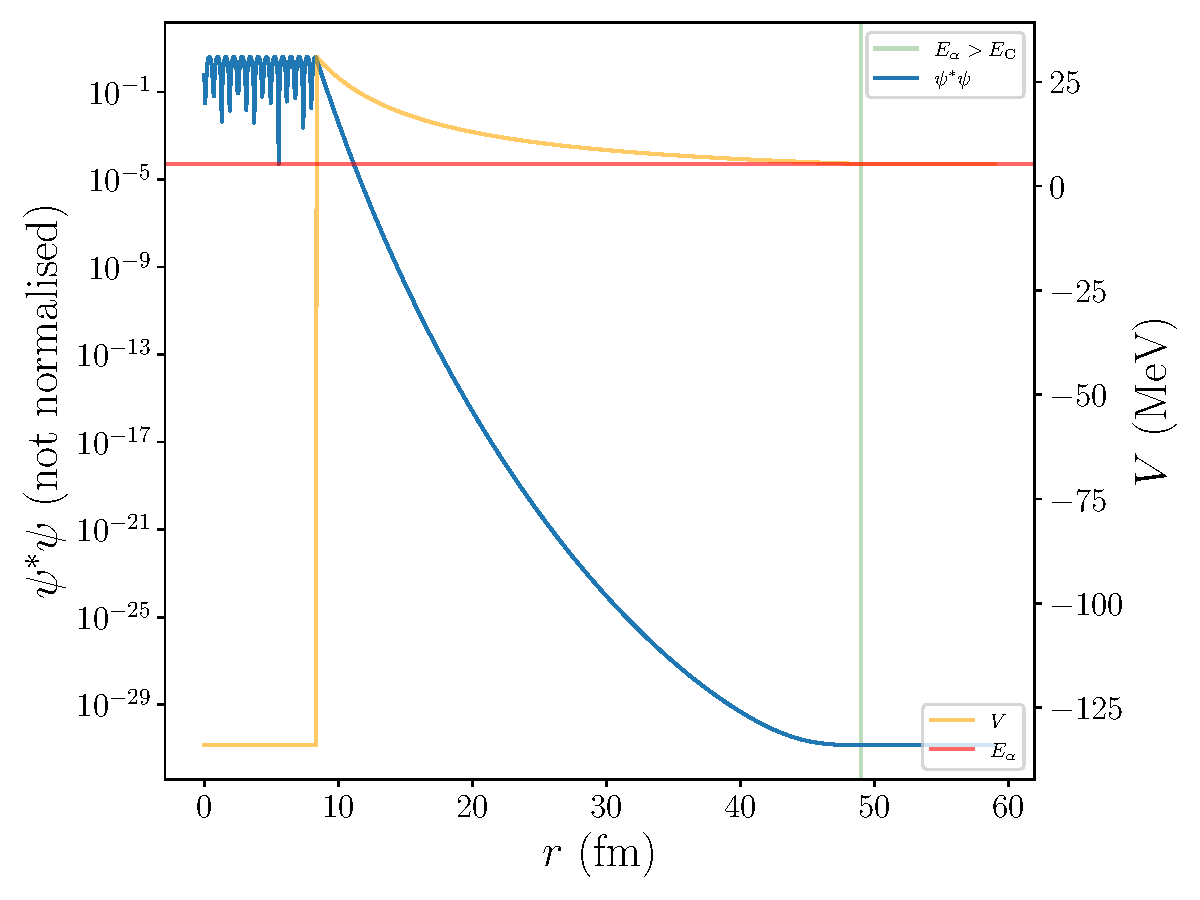
\includegraphics[width=0.9\textwidth]{../plots/density/u238.pdf}
        \caption{$^{238}\text{U}$}
        \label{subfig:density_u238}
    \end{subfigure}
    \begin{subfigure}{0.49\textwidth}
        \centering
        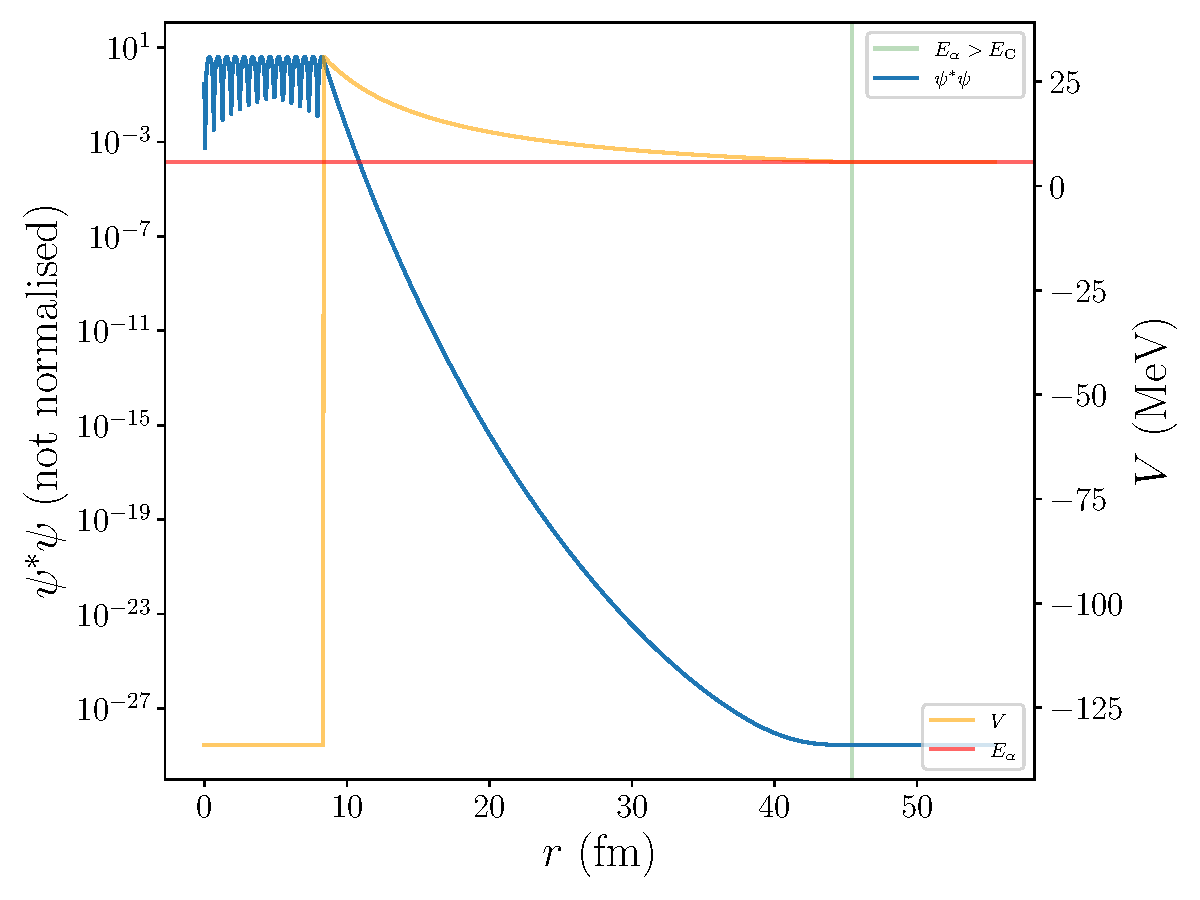
\includegraphics[width=0.9\textwidth]{../plots/density/u235.pdf}
        \caption{$^{235}\text{U}$}
        \label{subfig:density_u235}
    \end{subfigure}\\
    \begin{subfigure}{0.49\textwidth}
        \centering
        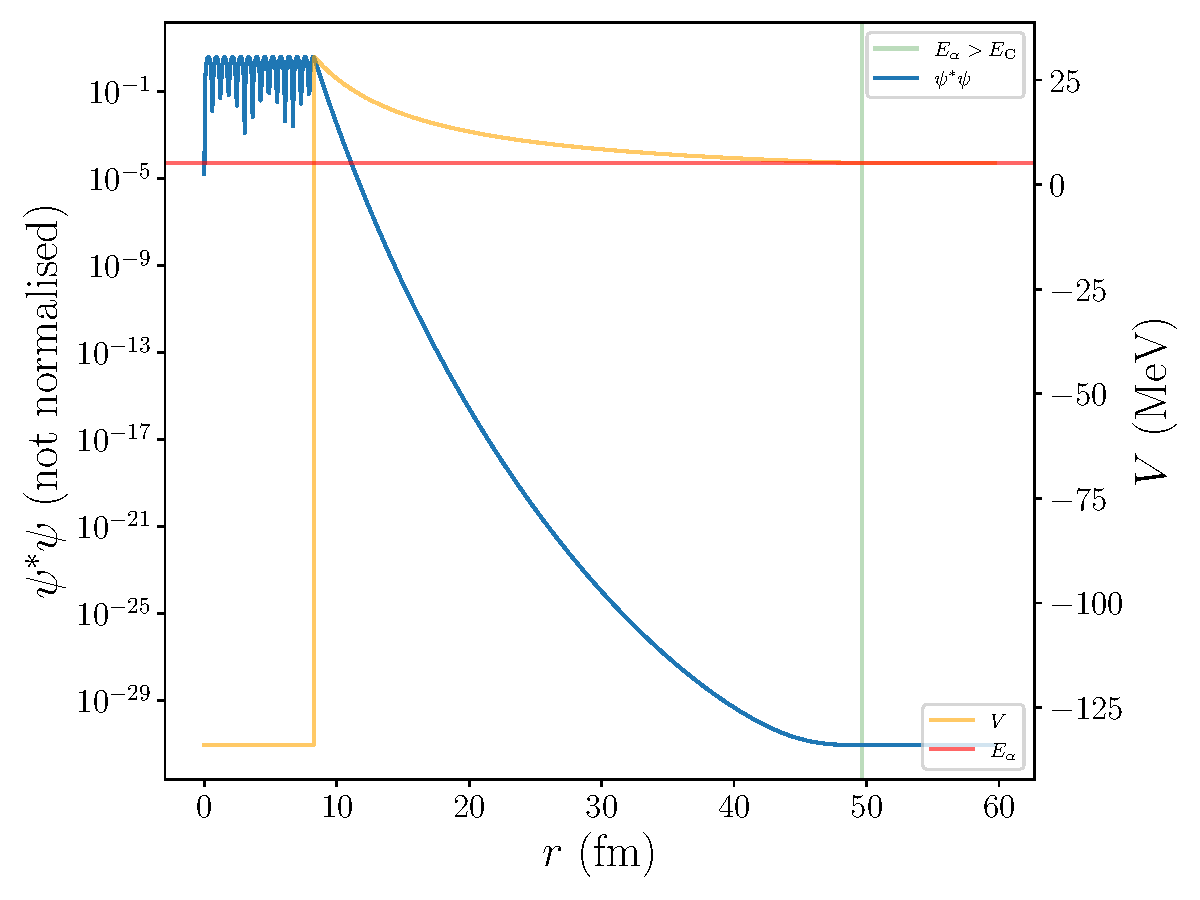
\includegraphics[width=0.9\textwidth]{../plots/density/th232.pdf}
        \caption{$^{232}\text{Th}$}
        \label{subfig:density_th232}
    \end{subfigure}
    \begin{subfigure}{0.49\textwidth}
        \centering
        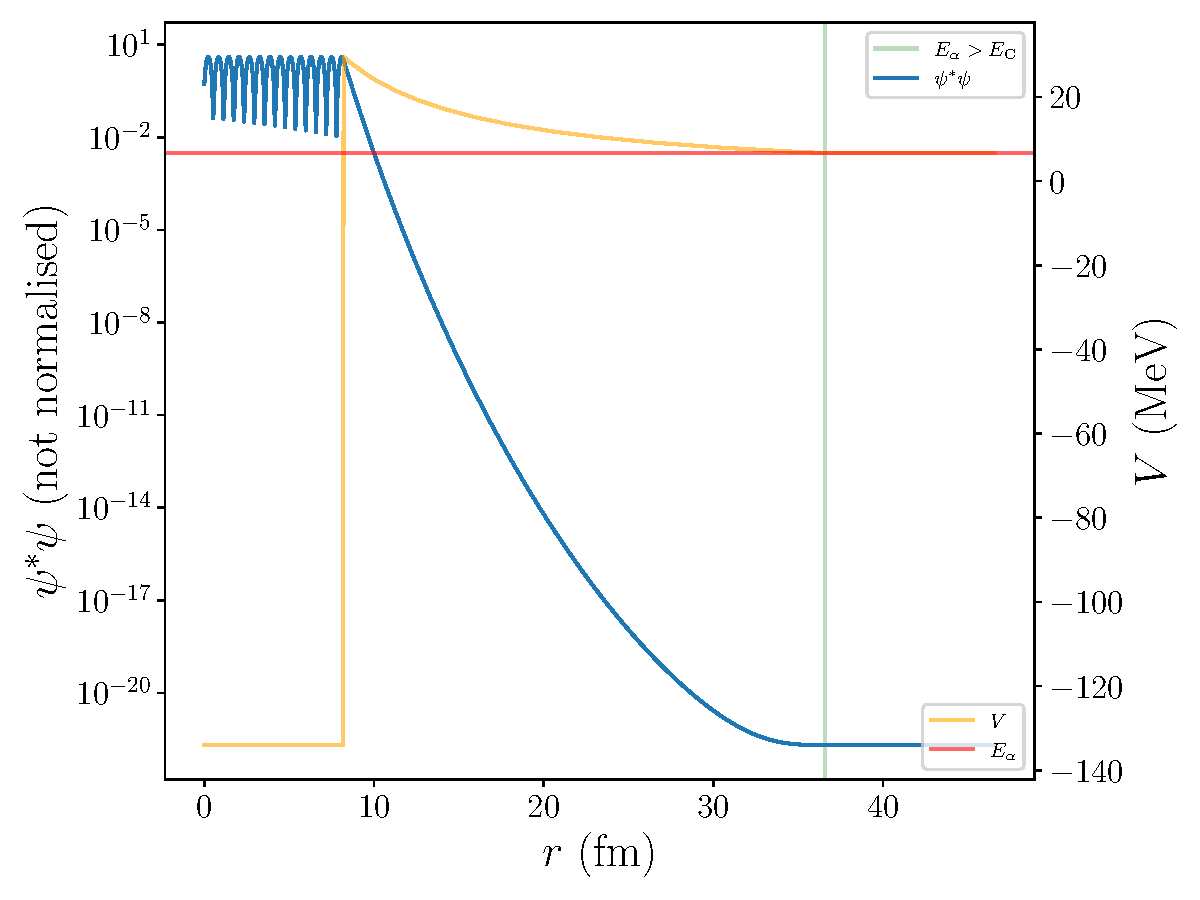
\includegraphics[width=0.9\textwidth]{../plots/density/rn222.pdf}
        \caption{$^{222}\text{Rn}$}
        \label{subfig:density_rn222}
    \end{subfigure}\\
    \begin{subfigure}{0.49\textwidth}
        \centering
        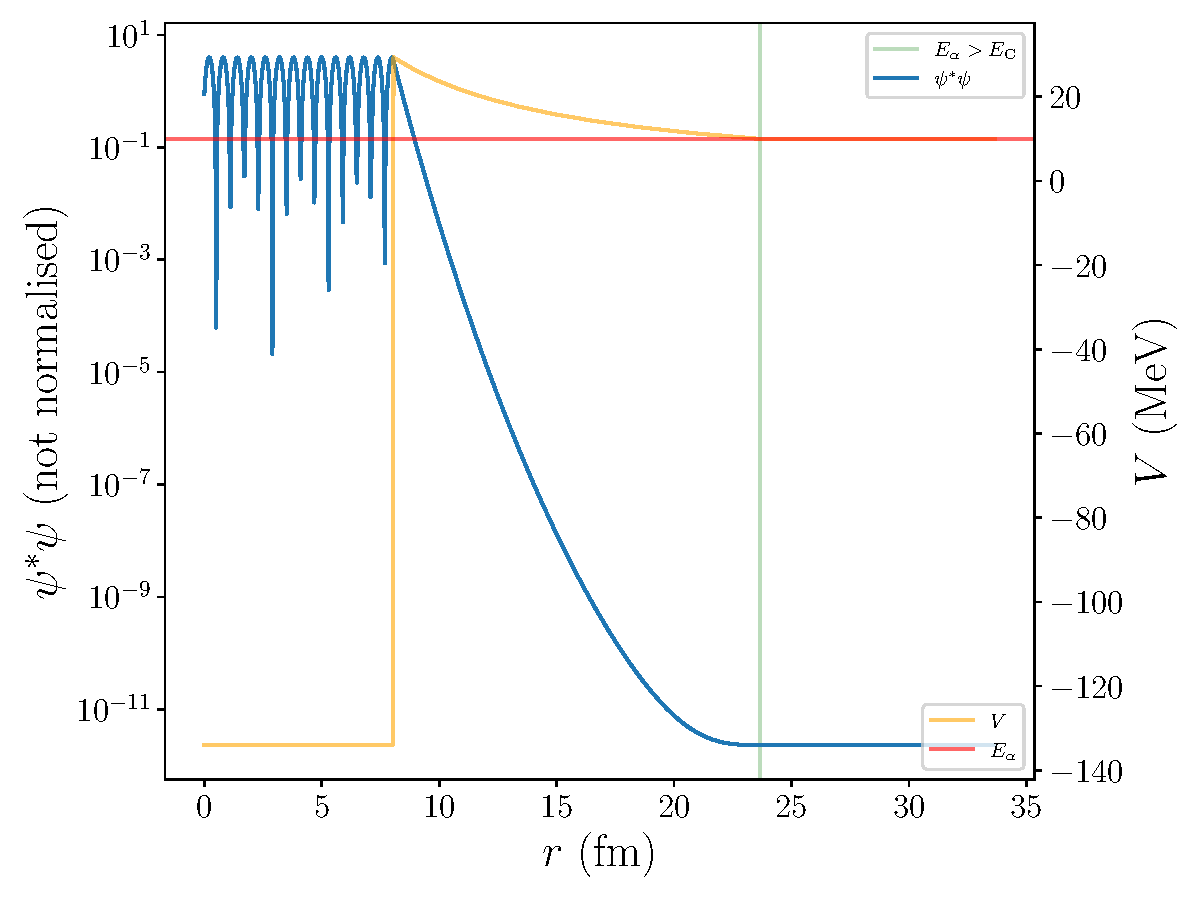
\includegraphics[width=0.9\textwidth]{../plots/density/po212.pdf}
        \caption{$^{212}\text{Po}$}
        \label{subfig:density_po212}
    \end{subfigure}
    \caption{Non-normalised squared absolute value of the wave function for the different isotopes. Parameters used: $\tilde R = 1.35$, $V_0 = - 134\,\text{MeV}$, 2000 bins. The wave function appears to be consistent with the continuity requirements imposed on it. The potential is also shown, here it is important to note that at $r=R_\text{C}$, the plot essentially assumes that the potential remains at a constant value and does not fall further.}
    \label{fig:density}
\end{figure}

\begin{figure}
    \centering
    \begin{subfigure}{0.49\textwidth}
        \centering
        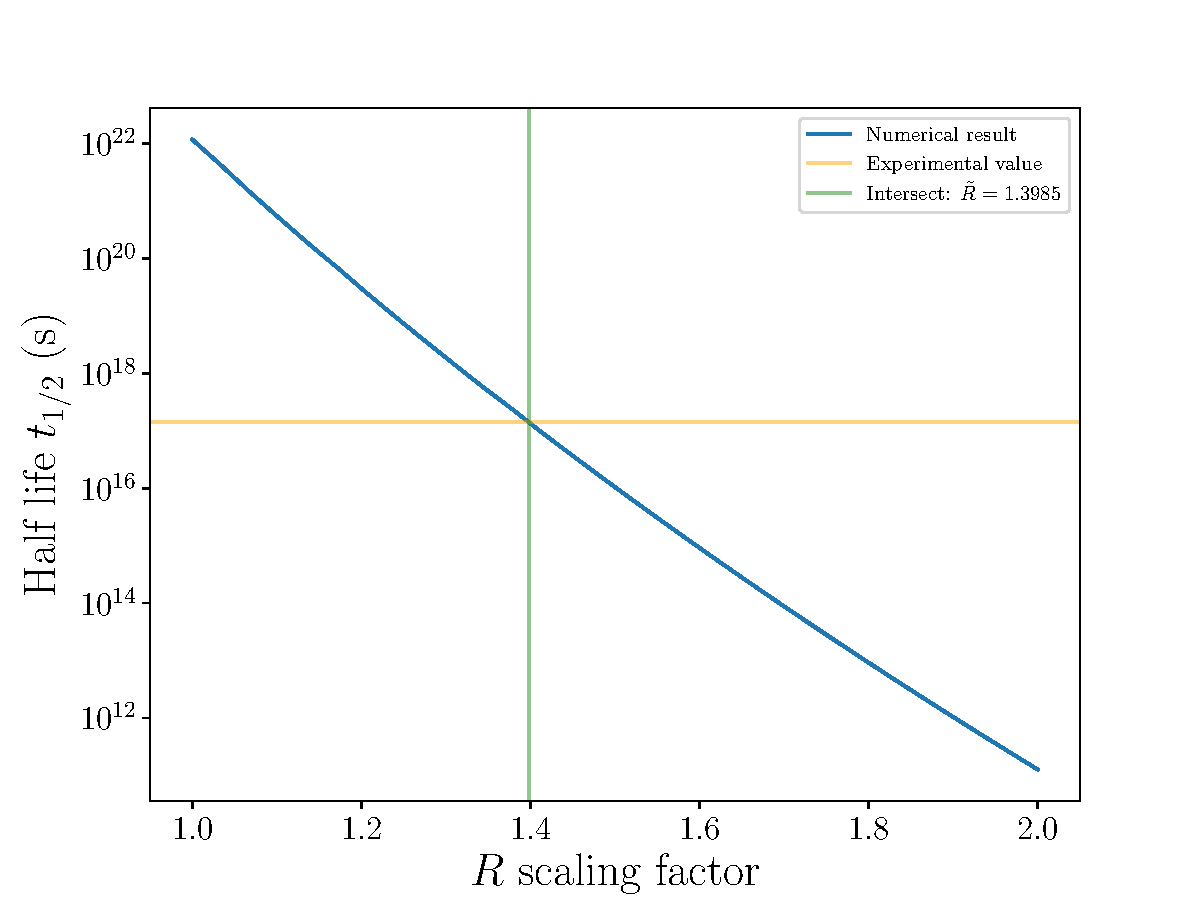
\includegraphics[width=0.9\textwidth]{../plots/R_dependence/R_u238.pdf}
        \caption{$^{238}\text{U}$}
        \label{subfig:r_u238}
    \end{subfigure}
    \begin{subfigure}{0.49\textwidth}
        \centering
        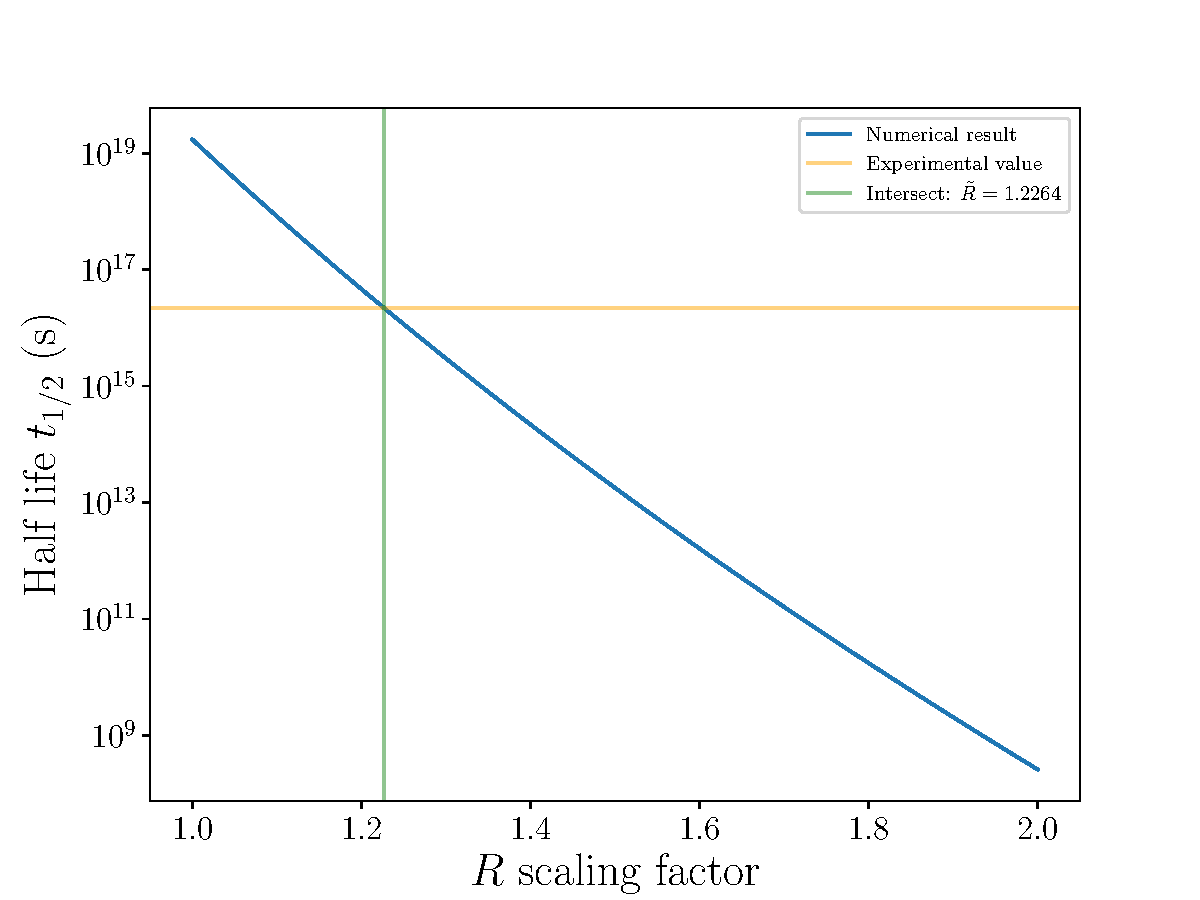
\includegraphics[width=0.9\textwidth]{../plots/R_dependence/R_u235.pdf}
        \caption{$^{235}\text{U}$}
        \label{subfig:r_u235}
    \end{subfigure}\\
    \begin{subfigure}{0.49\textwidth}
        \centering
        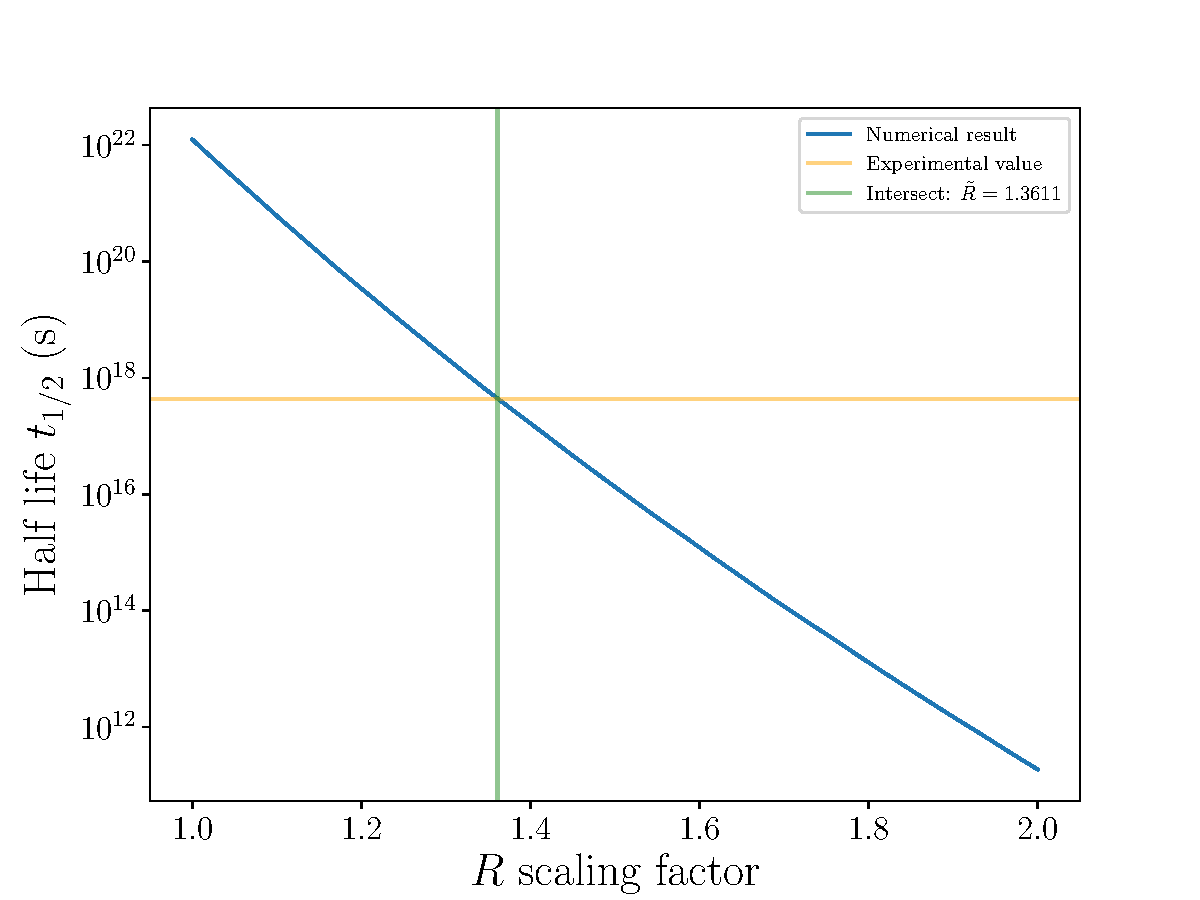
\includegraphics[width=0.9\textwidth]{../plots/R_dependence/R_th232.pdf}
        \caption{$^{232}\text{Th}$}
        \label{subfig:r_th232}
    \end{subfigure}
    \begin{subfigure}{0.49\textwidth}
        \centering
        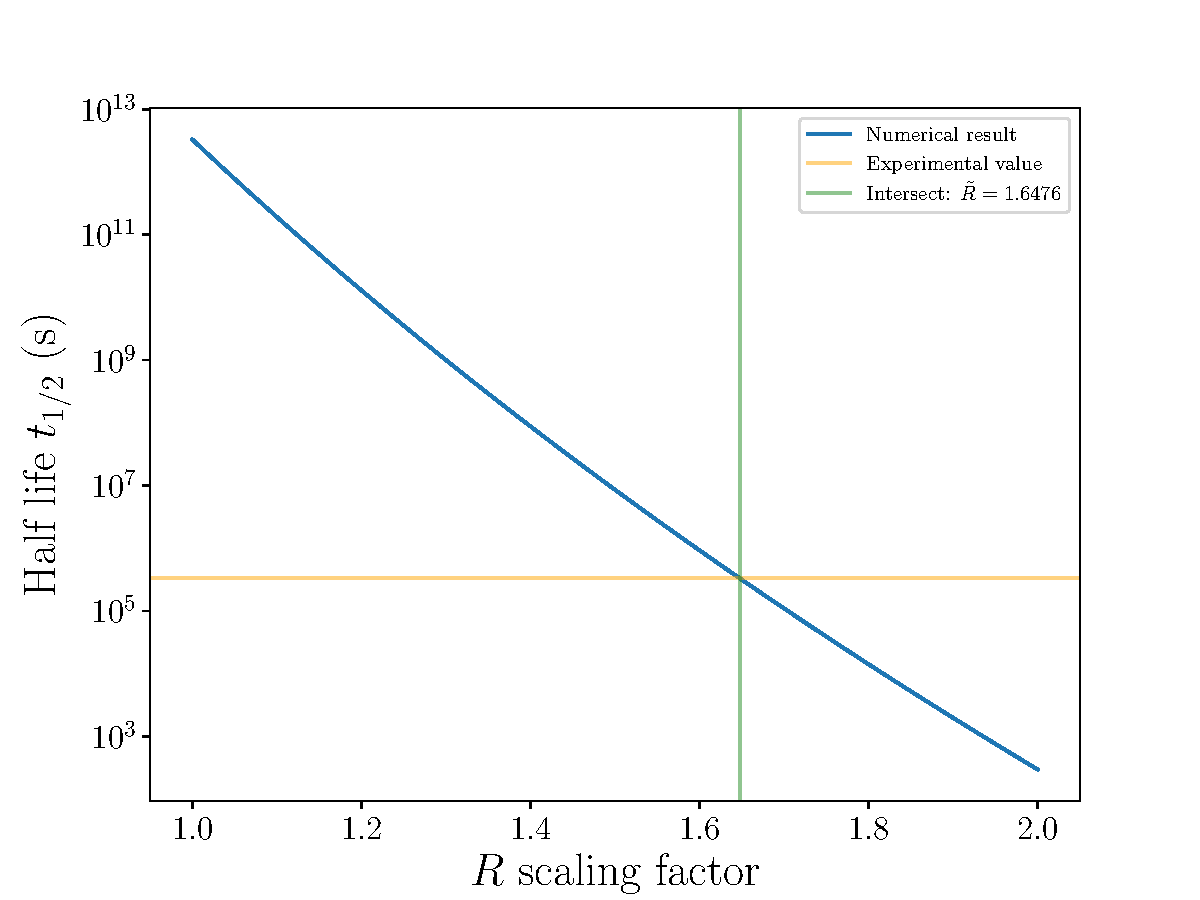
\includegraphics[width=0.9\textwidth]{../plots/R_dependence/R_rn222.pdf}
        \caption{$^{222}\text{Rn}$}
        \label{subfig:r_rn222}
    \end{subfigure}\\
    \begin{subfigure}{0.49\textwidth}
        \centering
        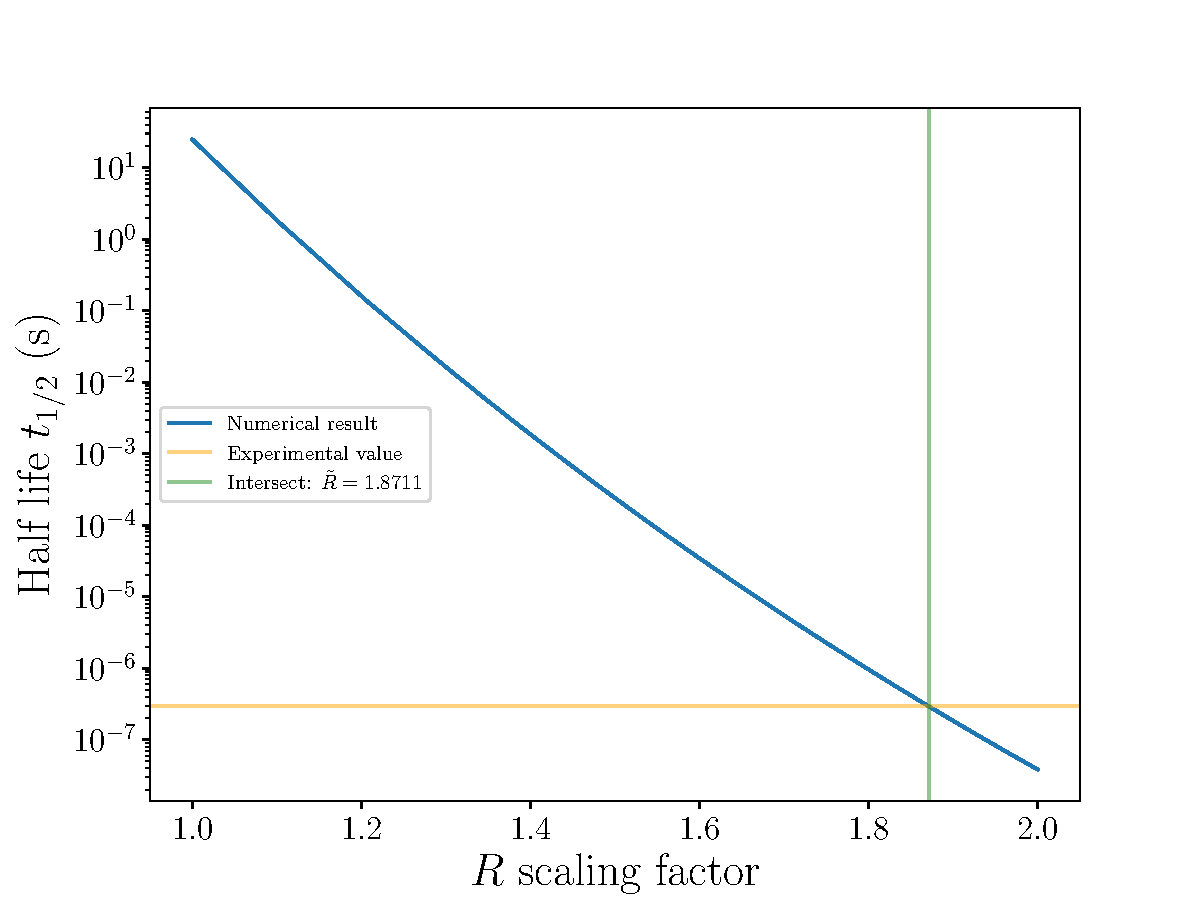
\includegraphics[width=0.9\textwidth]{../plots/R_dependence/R_po212.pdf}
        \caption{$^{212}\text{Po}$}
        \label{subfig:r_po212}
    \end{subfigure}
    \caption{Variation of the numerically estimated half life with the nuclear radius scaling factor $\tilde R$. The value of $\tilde R$ that reproduces the experimental half-life is indicated. For the Uranium and Thorium isotopes, this ranges between 1.25 and 1.4, which is why we chose to fix it to 1.35 for the rest of the analysis. For the lighter isotopes, the suggested $\tilde R$ approaches 2 which is most definitely unphysical.}
    \label{fig:r}
\end{figure}

\begin{figure}
    \centering
    \begin{subfigure}{0.49\textwidth}
        \centering
        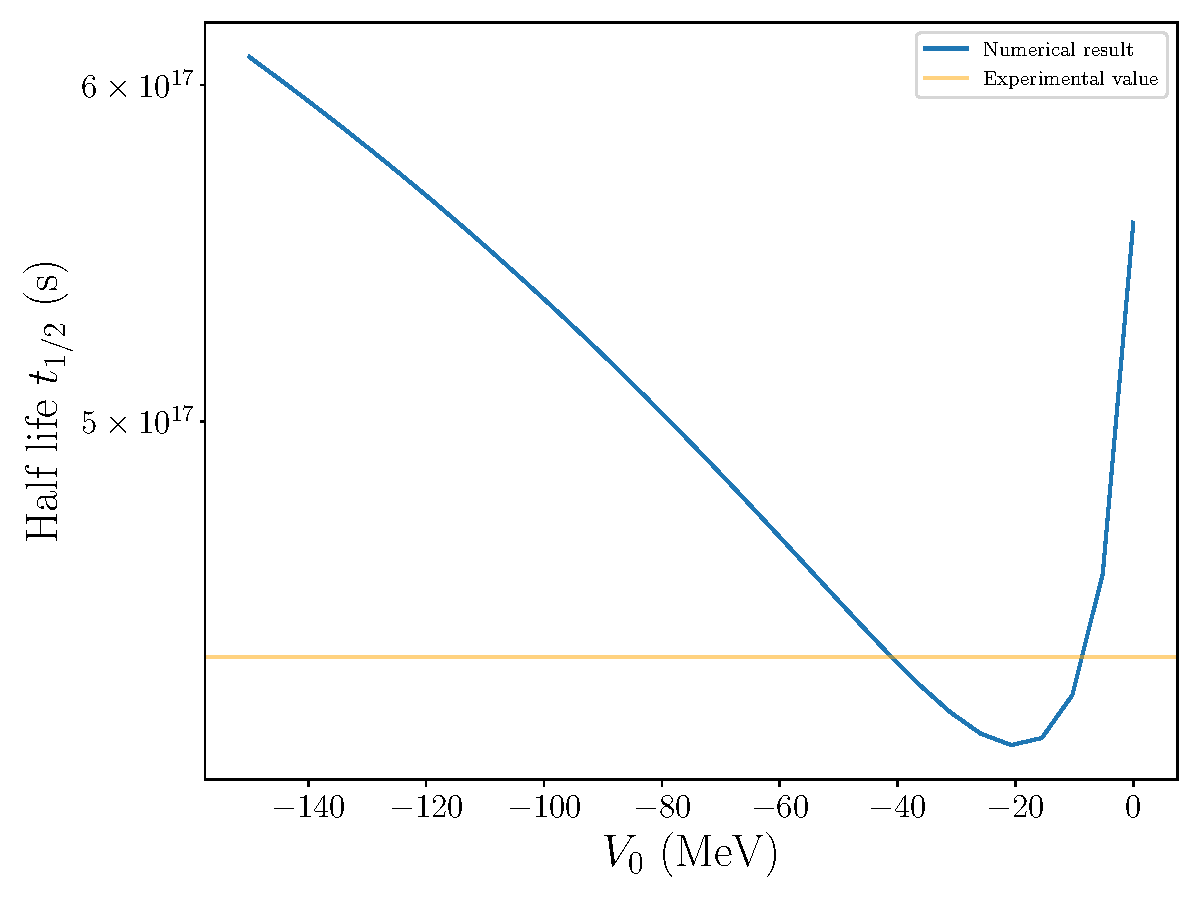
\includegraphics[width=0.9\textwidth]{../plots/V0_dependence/V0_th232.pdf}
        \caption{$^{232}\text{Th}$}
        \label{subfig:v0_th232}
    \end{subfigure}
    \begin{subfigure}{0.49\textwidth}
        \centering
        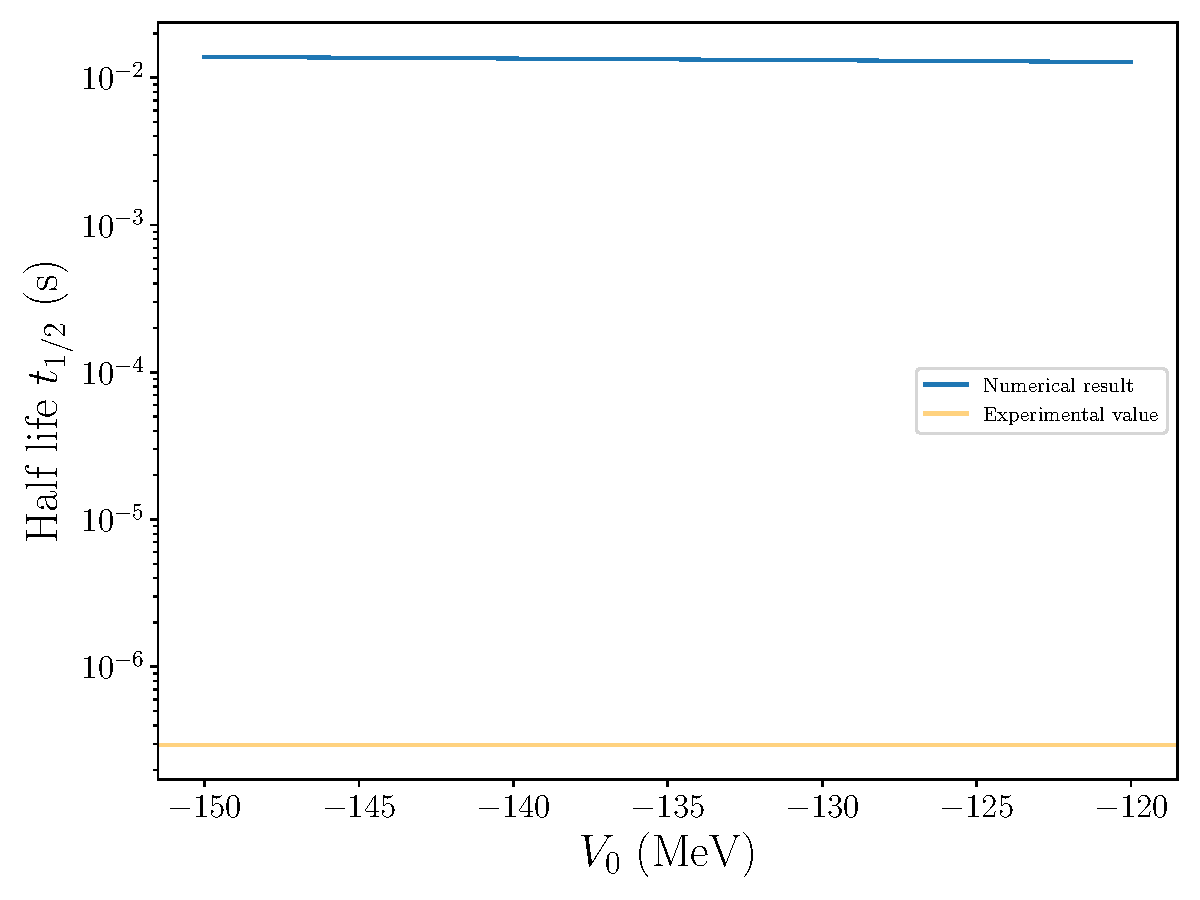
\includegraphics[width=0.9\textwidth]{../plots/V0_dependence/V0_po212.pdf}
        \caption{$^{212}\text{Po}$}
        \label{subfig:v0_po212}
    \end{subfigure}
    \caption{Variation of the numerically estimated half life with the depth of the potential well $V_0$ for two selected isotopes. It can be seen that, compared to $\tilde R$, $t_{1/2}$ varies slowly with $V_0$ even over a large range of potentials, one can not tune it such that the predicted half-lives agree with experiment.}
    \label{fig:v0}
\end{figure}

\begin{table}
    \centering
    \caption{Numerically estimated half-lives and relative errors with respect to experimental values.}
    \begin{tabular}{c|cc}
        Isotope & Numerical half-life (s) & relative error \\
        \hline
        $^{238}\text{U}$ & $4.68\cdot 10^{17}$ & 2.32 \\ 
        $^{235}\text{U}$ & $2.81\cdot 10^{15}$ & 0.87 \\ 
        $^{232}\text{Th}$ & $5.60\cdot 10^{17}$ & 0.27 \\
        $^{222}\text{Rn}$ & $2.83\cdot 10^{8}$ & 856 \\
        $^{212}\text{Po}$ & $1.31\cdot 10^{2}$ & 44500 \\        
    \end{tabular}
    \label{tab:result}
\end{table}

\begin{figure}
    \centering
    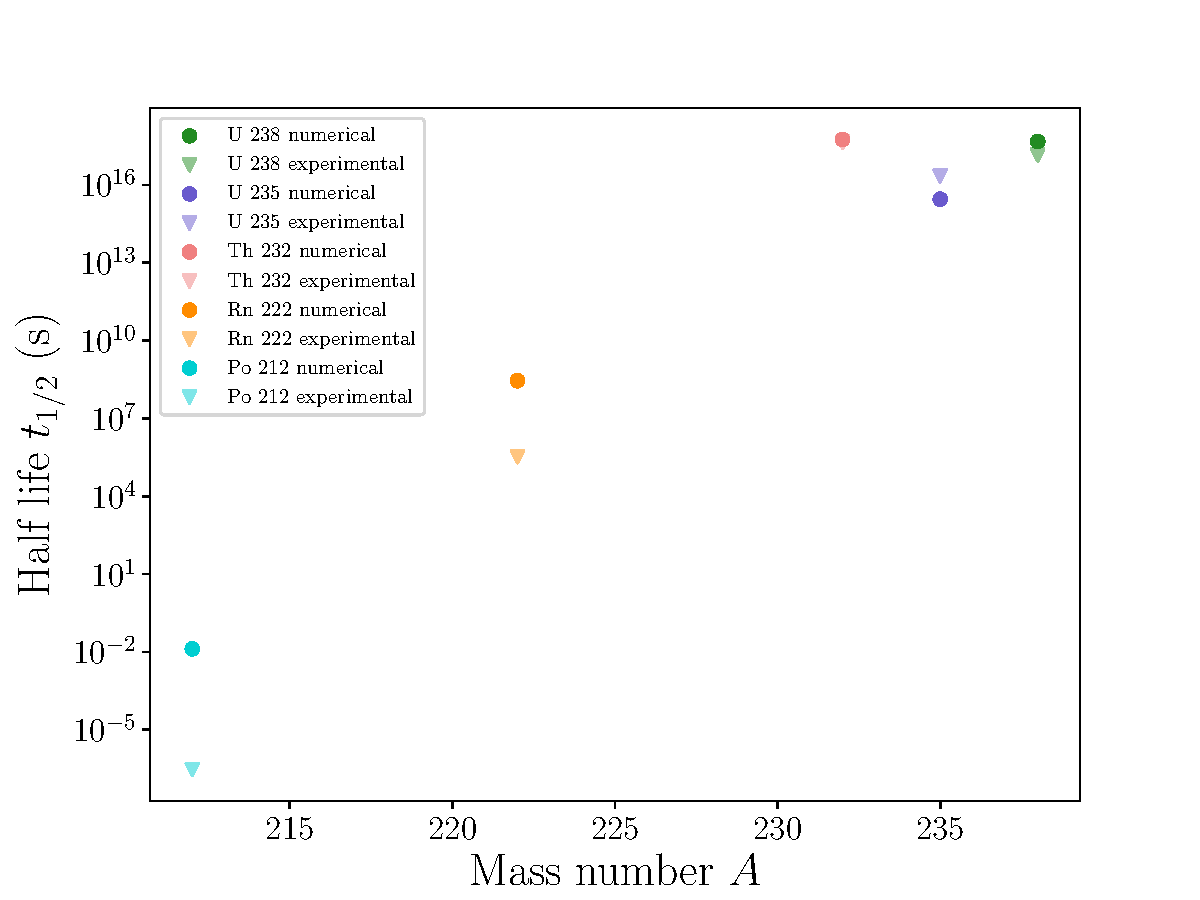
\includegraphics[width=0.8\textwidth]{../plots/summary_t.pdf}
    \caption{Summary of the best predicted values for the half-lives compared to experiment. Notably, the prediction for the heavy isotopes is within one order of magnitude. For the lighter isotopes, the error becomes larger as the value of the true half-lives becomes increasingly small. Notably, the model is able to reproduce the qualitative result that, within a small range of parameters, the half-life varies over many orders of magnitude. $^{235}\text{U}$ is the only isotope for which the predicted value is lower than the experimental one, this may be connected to the fact that it is the only odd-numbered isotope considered.}
    \label{fig:summary}
\end{figure}



\section{Conclusion}

\newpage
\FloatBarrier
\printbibliography


\end{document}
